%!TEX root = ../../dissertation.tex
%%%%%%%%%%%%%%%%%%%%%%%%%%%%%%%%%%%%%%%%%%%%%%%%%%%%%%%%%%%%%%%%%%%%%%%%%%%%%%%
\chapter{Introduction}
\label{chap:intro}


\begin{itemize}

\item ARPANAT and evolutionary process to today's Internet scale
\item outside and inside developments brings new Internet usage (mp3+p2p, bandwidth+codecs -> video, digicams/camcorder); socioeconomic developments of a free speech network;New traffic patterns emerging due to external developments. Digital cameras, new codecs (esp MP3, mpeg4, WebM) -> p2p, Webcams 
\item mobile networks: more of a parallel development to the Internet, always centralized (from the old copper/telephony/circuit switched world)
\item MNs very different to the Internet structures we are used to
\item circuit switched roots, signaling, explicitly NOT a distributed system as compared to Internet, i.e. explicit signaling central controllers
\item Streaming and Multicasting, Multicasting in the Internet in general (only somewhat relevant for live/realtime non-interactive stuff)
\item  network intelligence at the end nodes
\item --> end-to-end violations: ECN? only signaling, decision is e2e, same category as indirect TCP congestion control signaling (through loss) from the network; NAT, Firewalls?
\item content agnosticism: we do not know what applications the future will bring, so we do not make any assumptions
\item HTTP; ``The Web adopts relatively simple technologies with sufficient scalability efficiency and utility'' \cite{W3Arch}
\item Why HTTP streaming? Generalization of HTTP streaming (reliable transport, control shift to the client); Less control, more effective; Why global QoS control doesn't work
\item LTE, EPC, Core network tunneling concepts, bottlenecks in the access and the core, LTE network model
\item Improvements to congestion control for mobile streaming
\item Influence of L1/2/3 layer protocols and mechanisms (IPv4/6, tunneling, ethernet vs RLC/RRC/NAS, ...) ; what works better with it? compare, model and measure
\item QoE metrics, MOS, stalling time and buffering models, subjective and objective testing
\end{itemize}

%% new thesis stuff
Packet Switching, the process of chunking information into smaller bits, labeling it and transmitting it independently, was first described by Paul Baran in the 1960s\cite{baran1964distributed}. This changed communication a lot and provided one of the foundations for the emergence of the Internet. 

The original usage intent was mostly limited to remotely logging into and communicating with mainframe computers and transferring files supported by the emergence of new multiuser and multitasking operating systems, especially including the release of UNIX in 1969.\todo{needs references}

From these early times countless other services and applications emerged. Today, the Internet is by used hundreds of millions of people, touching almost every aspect of daily life. The creation of the World Wide Web -- begun by Tim Berners-Lee in 1989\todo{reference} -- brought an easily accessible ``user interface'' to the Internet and made adoption for the masses much easier. Today, almost any form of application is available through the Web as a combination of \ac{HTML}, \ac{CSS}, and JavaScript and can be accessed by just opening a Web browser.

But as is the case with many technological fields, the Internet's development was also closely entangled with other advancements. Take the huge Internet music wave beginning in 1999 as an example. It may have been started by the creation of Napster, the first peer-to-peer file sharing service. However, without the large improvements in audio compression -- namely MP3 -- a few years before, including computers that could handle decompression as well as compression and increasing Internet access bandwidth (and fixed service fees) , this would not have been possible. Similarly, YouTube could not have existed without a wide spread of digital camcorders and many other devices with recording capability, good video compression codes, and an even further increase in access bandwidths.
 For every leap in bandwidth new services sprung to life fueling the users' demand for further capacity increases. 

% content agnosticism: we do not know what applications the future will bring, so we do not make any assumptions

Several factors contributed to the quick acceptance of the Internet. First and foremost no assumptions are made on the transported content, or content agnosticism. The original idea is to treat every packet, every participating node the same and do not make any assumptions on specific applications. This provides a level playing field for every contender wanting to offer services. This is upheld by the second driving concept, the ``End-to-End Principle'', \cite{saltzer1984end2end} stating:

\begin{quote}
``The function in question can completely and correctly be implemented only with the knowledge and help of the application standing at the endpoints of the communications system. Therefore, providing that questioned function as a feature of the communication system itself is not possible. [...]''
\end{quote}

End-to-End means that any functionality, meaning services or applications, should only be implemented at the two endpoints of a transmission not somewhere in between. Tuning the network to specific applications and implementing functions inside the network, will always only be valid for existing and narrow use cases and cannot support future developments.

During the past decades this has often been discussed  \cite{bhattacharjee1997active, blumenthal2001rethinking, isenberg1997rise, lemley2000end} but is still being upheld for the most part for good reason. \todo{probably should clarify the good reason}. This is in contrast to the way telephone networks and their operating companies historically worked. These networks are based on circuit switching and access as well as content (namely voice calls) and procedures are tightly controlled by the operator.
%\\

%%%%%%%%%%%%%%%%%%%%%%%%%%%%%%%%%%%%%%%%%%%%%%%%%%%%%%%%%%%%%%%%%%%%%%%%%%%%%%%%
\section{Video and the Internet}

\begin{figure}[htbp]
    \centering
    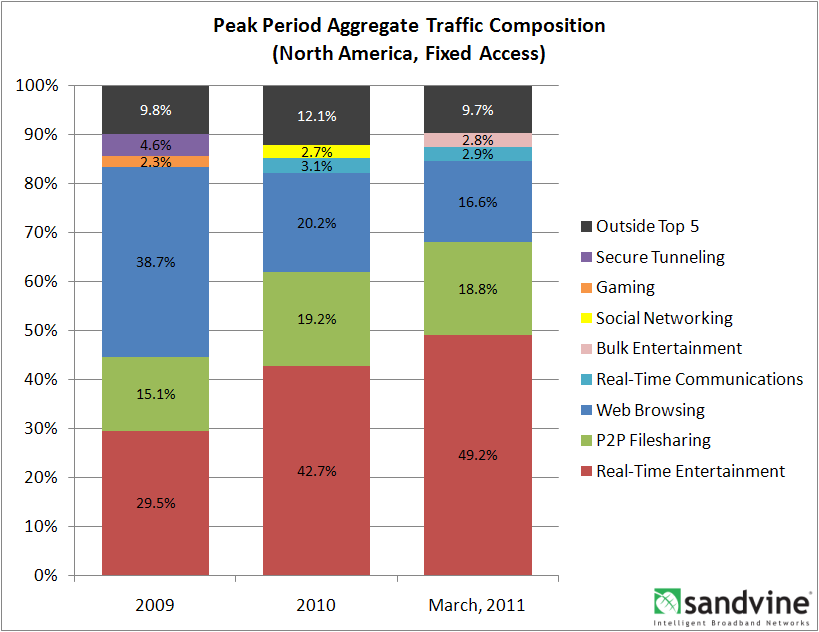
\includegraphics[width=0.8\textwidth]{images/netvine.png}
    \caption{Netvine, North American peak traffic (Source: \cite{sandvine_spring2011,sandvine_spring2013}).}
    \label{c1:fig:traffic_netvine}
\end{figure}

\begin{figure}[htbp]
    \centering
    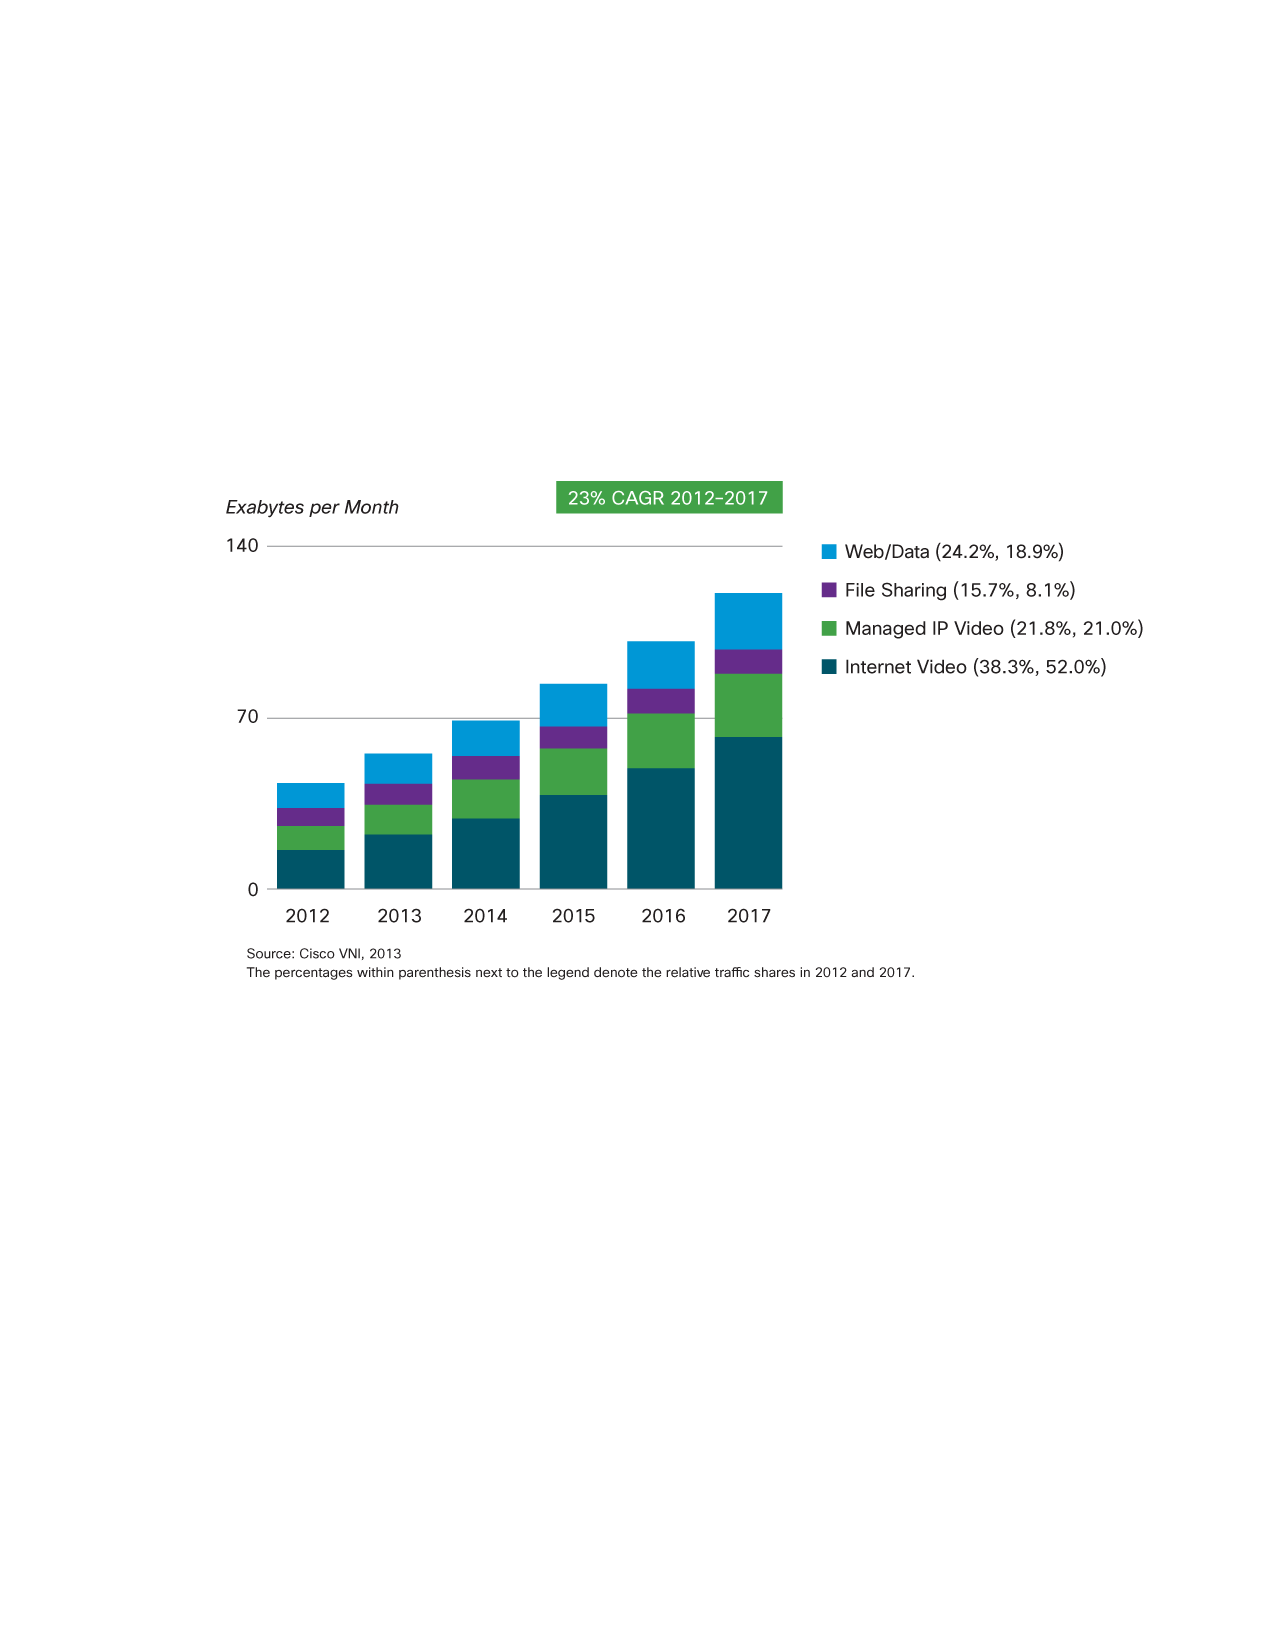
\includegraphics[width=0.8\textwidth]{images/VNI_Hyperconnectivity_WP.pdf}
    \caption{Cisco, global consumer Internet traffic prediction (Source: \cite{cisco2013VNI}).}
    \label{c1:fig:traffic_cisco}
\end{figure}

The total volume of Internet traffic has been rising exponentially for many years. The composition of today's traffic is manifold, but one of the largest contributing factors is arguably video (take a look at Figures~\ref{c1:fig:traffic_netvine} and \ref{c1:fig:traffic_cisco}). Studies predicting the development of the Internet's traffic also tell of the large influence of video in the near future. The two main sources for this video are YouTube\footnote{\url{https://www.youtube.com}} and, in countries where its available, Netflix\footnote{\url{https://www.netflix.com}}, and even newer services like the live-streaming site Twitch\footnote{\url{http://twitch.tv}} acting as runner-up.

Despite not wanting to tune the network to video, it is still very important to understand the dynamics happening around this type of traffic there. With a traffic portion this large any events or behavior specific to this portion will also have a huge impact on the total network.
Transporting this video -- or rather ``streaming'' as in watching the video while it's still being transmitted -- -- integrating themselves much better into the current Web ecosystem --  in the Internet has again become a topic of hot discussions. There are long-standing application layer protocols for exactly this use case. \ac{RTP}, as the most prominent, has been described as early as 1996 \cite{rfc1889}. It is well described in standard educational literature and specifics to it are still being researched and improved on. Interestingly however, it is practically not being used at all in the current updraft of video traffic. \todo{explain the reason (Web-relationship, tcp basis, firewalls, walled gardens, ...)either here or in a later chapter}
Instead, new approaches have been thought out, integrating themselves much better into the current Web ecosystem.
And they are using completely different modes of transportation and control. Streaming, and media transport in general, is also not only relevant for the purpose of watching videos, there are many more fields of use with similar requirements. Becoming popular in the last years is the so-called Cloud Gaming: Running virtualized video games on large racks and streaming just the video output to the clients with all the user input handled by the server, putting a huge emphasize on achieving low latency.\footnote{Select works overviewing this thematic complex are, e.g., \cite{4795441,wang2009modeling,jarschel2011cloudevaluation,ct2010wolken}.}
Investigating the implications coming with these new streaming protocols will be the first task of this thesis.
%\\

%%%%%%%%%%%%%%%%%%%%%%%%%%%%%%%%%%%%%%%%%%%%%%%%%%%%%%%%%%%%%%%%%%%%%%%%%%%%%%%%
\section{The Network Below}

Looking back to the actual networks, we also see lots of progress in the past. Despite their rapid evolution, mobile networks, however, still carry much heritage from their circuit switching roots. \footnote{For an historical overview refer to \url{https://en.wikipedia.org/wiki/History_of_mobile_phones}. \todo{should remove wikipedia}}
Starting in the 1950s with early analog predecessors like the German ``A-Netz'' and first generation cellular structured networks in the eighties, mobile telephony entered the fully digital world with the European \ac{GSM} and competing \ac{CDMA}-based technologies around the year 1991. This was similar to the development in the \ac{POTS} with its shift away from the analog roots to digital circuit switching technologies like \ac{ISDN}.

Because of its huge success \ac{GSM} and its packet-switching extension \ac{GPRS} was used as a blueprint for the following mobile network standard evolutions resulting in \ac{UMTS} (including \ac{HSPA} and \ac{HSPA+}), today's \ac{LTE} and even the upcoming \ac{LTE} Advanced. Through this heritage, many network elements and protocol have hardly changed since the beginning and are still strongly connection orientated with a strong tendency to signaling and statefulness.
This creates a wide range of problems which have only begun to show up in recent years due to the large influx of new user and usage scenarios, creating traffic patterns unheard of a few years ago and overwhelming the network's control plane structures. 

%% still WIP
Traffic in cellular networks follows a development similar to that of the Internet as a whole as described earlier. Through the advent of affordable high performance smartphones, thriving mobile application ecosystems, and (relatively) fast access technologies many are now using their phones as the primary device for interacting with the Internet. This includes the same bandwidth consuming services as in fixed access 

Combined, these facts pose unique challenges and opportunities for the design and dimensioning of network protocols. Adding to this, is the circumstance, that mobile networks and mobile network equipment is usually regarded as trade secrets by 
Little is known of the exact make-up of these networks as they are closely guarded secrets of the operator.
This presents us with the second task of this thesis.

This can put pressure on the overly complex cellular network structures. The radio transmissions have only access to a limited radio frequency spectrum that, moreover, has to be shared with any other phone user in the same cell. But there is also deemed to be significant pressure on the traffic management mechanisms of the mobile core networks backing up and aggregating the numerous radio cells of an operator. 


%%%%%%%%%%%%%%%%%%%%%%%%%%%%%%%%%%%%%%%%%%%%%%%%%%%%%%%%%%%%%%%%%%%%%%%%%%%%%%%%
\section{Research Motifs and Goals}

%% <--



The topic of the thesis will be the research of the inner workings of these new streaming services and mechanisms and especially its impact on the aforementioned cellular core network structures. This means conducting performance evaluations of the streaming mechanisms on itself and in the context of mobile networks as well as performing systematic assessments and classifications of the mechanisms. 

The result will be an understanding of the quantitative attributes related to these new forms of streaming. Furthermore, the thesis should provide tools and methods that help decide all participants of media streaming and mobile network operators which protocols and methods to choose and which are best suited for specific applications


%TODO:
    Performance analysis and comparison model of existing media streaming solutions
      But do not compare the protocols but the mechanisms and paradigms behind it
    Special focus on mobile environments and their pitfalls
    Improvements to protocols and new approaches

    Neue Videostreamingtechniken sind beliebt und bringen immer mehr Last in Mobilfunksysteme. Die Leistungsfähigkeit und die Qualität der Streaming-Dienste hängt insbesondere vom Verkehrsmanagement in Mobilfunksystem ab. Die Arbeit soll die Leistungsfähigkeit der neuen Streamingverfahren in heutigen und zukünftigen Mobilfunksystemen, die mit dem Internet verbunden sind, untersuchen. Die Schwierigkeit der Arbeit besteht in der Komplexität der Mobilfunksysteme und der neuen Streamingverfahren sowie in der Verknüpfungen der beiden Konzepte. Insbesondere die Auswirkung der Mobilfunkkernnetze auf die Leistungsfähigkeit der Mechanismen der Transportschicht sollen mit Hilfe von Methoden aus der Leistungsbewertung von Rechner- und Kommunikationsnetzen, untersucht werden.


On which kind of network information flow should streaming applications rely on in general and mobile networks specifically? What information is actually required for streaming?

What information flow should be provided by networks?

How can and should information be exchanged?

Can or should there be any dependence of the information flow on the application layer protocol?

How can the information flow be evaluated and modelled and the protocols and network architectures be compared? Is a generic evaluation model possible?

Design of new transport or streaming mechanisms
-> Formal Description Techniques

-> Analytical Tool, test viability


%%%% end work-in-progress text -->


Concepts for future Internet structures are strongly disputed at the moment. A vast array of concepts is under discussion to either replace or enhance the protocol stack of the Internet's current setup. It will be interesting to measure the influence on media streaming and transport of these proposed changes or if there is any influence at all.








%%%%%%%%%%%%%%%%%%%%%%%%%%%%%%%%%%%%%%%%%%%%%%%%%%%%%%%%%%%%%%%%%%%%%%%%%%%%%%%%
\section{Solution Spaces}


\begin{figure}[htbp]
    \centering
    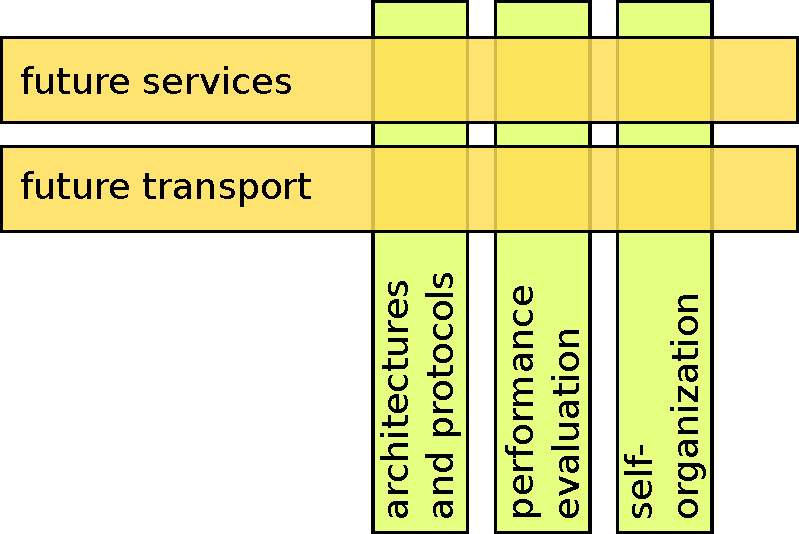
\includegraphics[width=.8\textwidth]{images/hv-topics-new.pdf}
    \caption{Technical solution spaces to the problem layers.}
    \label{c1:fig:hv-topics}
\end{figure}

As discussed, the core problems are layered into services and transport. Technologically, to solve the tasks of video streaming, one can approach these  threefold as displayed in Fig. \ref{c1:fig:hv-topics}.

The first is to dissect the involved protocols and architectures and break them down into their functional and methodical components. This will result in an improved understanding on the manner and process of their implementation. These components serve as building blocks for generalized models that abstracts the problem space from the actual implementation. The model will be defined by a set of parameters. To explore viable parameter ranges performance evaluation methods will be facilitated.


Secondly, using performance evaluation a system is methodically tested to the outcome of determining the influence of the system's parameters on a set of performance metrics. The parameters can be categorized into system intrinsic parameters, describing behavior only relevant and observable inside the system, and external parameters. In communication networks a good example for external parameters are the network Quality of Service parameters including latency, loss, jitter, and bandwidth capacity. Identifying fitting metrics for the measurement is a challenge. They can be either subjective or objective. The former are called Quality of Experience (QoE) metrics. They can only be measured by conducting empirical user studies and questionnaires and are mapped to a Mean Opinion Score (MOS). Extensive work has already been done to define baseline references for QoE metrics. Using these, one can directly translate objectively measurable outcomes into QoE metrics. However, these mappings may need to be adjusted to be able to handle stalling as the main source of quality loss. Examples for measuring subjective quality are available in \cite{gustafsson2008measuring, ketyo2010qoe}. 
Finally, one could employ methods of self-organization to try to reach improvements over conventional network setups.


\subsection{Apparatus for System Analyses and Comparison}

\begin{figure}[htbp]
    \centering
    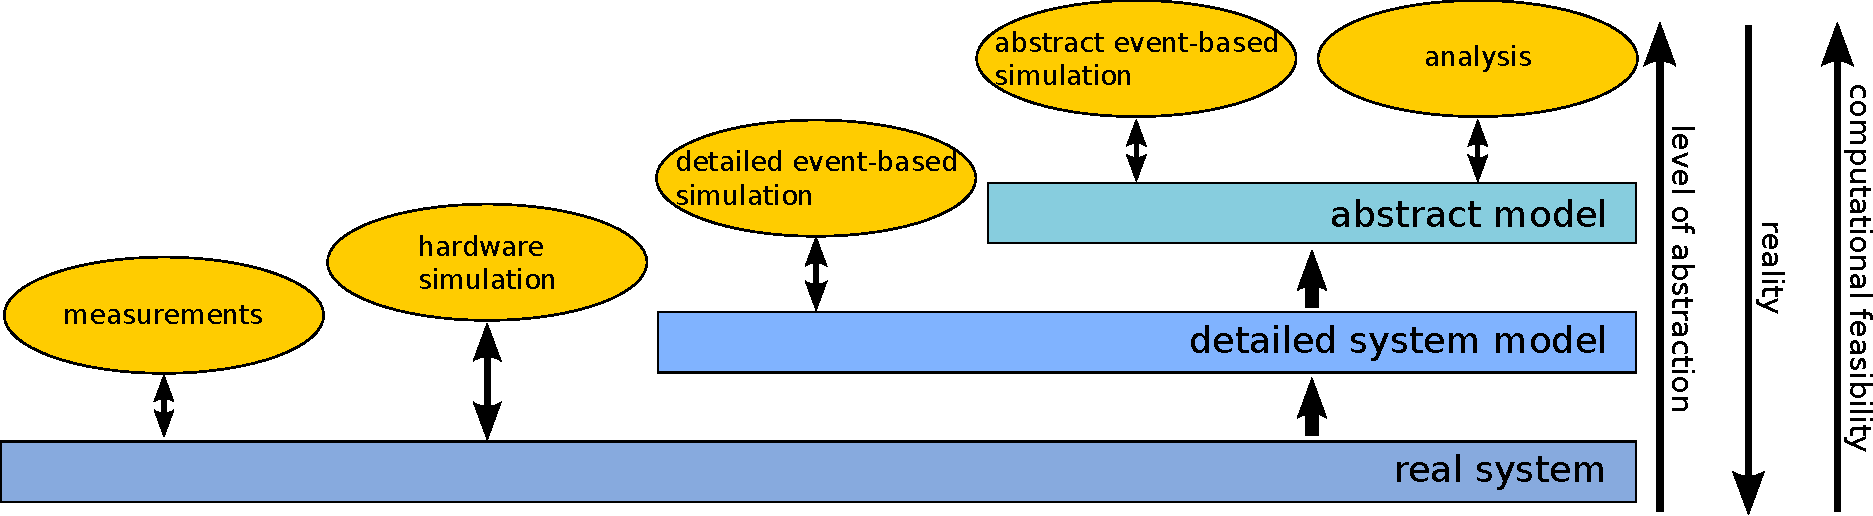
\includegraphics[width=1.0\textwidth]{images/apparatus-new.pdf}
    \caption{Methodical solution spaces and apparatus comparison.}
    \label{c1:fig:appcomp}
\end{figure}

Depicted in Figure \ref{c1:fig:appcomp} are levels of abstraction involved in system analysis and possible approaches to understand the system involved.

The upper limit for precision is achieved through actual measurements of the system itself. These give a point of reference and can be used to validate all other methods. However, this is not feasible to ascertain a larger view. The time frame or the physical size of the system is always limited.

Aside from measurements on implementations there are three further possible approaches which can widen the scope: emulation, simulation and mathematical analysis. 
Emulation tries to resemble implemented functionality as closely as possible while reducing the non-important parts to a minimum. Measurements using emulations can run in a normal network environment testbed and thus can only be done on a scale equivalent to implementations. The simulative approach implements all internal and external functionality, including the physical nodes and the network, in a discrete event simulation (DES). There may be subtle functional differences between a simulation and a real implementation. Therefore, validation is required. This approach benefits from the decoupling of the simulation from physical nodes as well as real time, allowing to measure large-scale networks in a short amount of time.
A mathematical analysis, for example using queuing theory and stochastic models, can then further broaden the understanding of the system.


The methods can all be used to define and explore solution spaces and are therefore important tools in understanding the problem. A fitting combination of these tools has to be found to advance the research. Our initial approach is to investigate existing streaming services, YouTube \cite{metzger2011delivery,mok2011measuring} and,e.g., video libraries of broadcast stations for simple HTTP streaming. A suitable candidate for measuring adaptive streaming still needs to be found as some candidate services apply regional restrictions. There are several reference applications available that implement different standardization approaches. These can be used to either directly measure the performance or to setup an emulation model based on their specifications.


\subsection{Further Approaches}
Further approaches which are under consideration, but will not be presented in detail here, are:

\begin{itemize}
\item Application of analytic and stochastic methods.
\item Formal definition of protocols or systems using Finite State Machines (FSM).
\item Creation of equivalent models.
\item Application of queuing theory, modeling the system through arrival processes, service time distributions and a number of servers and waiting places.
\item Data-mining of network trace data from mobile networks.
\end{itemize}



\subsection{Architecture and Protocols}

Mechanisms and protocols for the future of media streaming

\begin{itemize}
\item Compensation mechanisms for reliable transport
\item Model and quality estimations for improvements to adaptive streaming
\item End-to-end encryption and Authentication mechanisms (e.g.IPSec, DNSSEC, CurveCP) %(Daniel J. Bernstein)
\item Modifications to and issues with TCP
 \begin{itemize}
 \item TCP buffer bloat
 \item Initial window size (IW10, ...)
 \item WebSockets as streaming transport \cite{w3c2011websockets} \cite{heise2011websockets}
 \item WebRTC
 \item Relevance of multicasting or similar techniques for streaming transport (real-time live vs. stored)
  
 \item
 \end{itemize}
\item Service discovery and positioning (DNS modifications, CDNs, URIs, ``networking named content'')
\item Mobile networks
 \begin{itemize}
   \item Loss Hiding and conflict with congestion control mechanisms
   \item Shared media access, streaming with bandwidth/delay variations
   \item Mobility issues
     \begin{itemize}
       \item Mobility as a delay and loss source and its influence
       \item Investigation of mobility awareness and prediction techniques ("unassisted mobility")
     \end{itemize}
   \item future mobile networks
     \begin{itemize}
       \item Influence of control planes % Remove/Merge Control and User Plane
       \item Influence of (core) network elements (or a reduction thereof)
     \end{itemize}
 \end{itemize}

\end{itemize}




%%%%%%%%%%%%%%%%%%%%%%%%%%%%%%%%%%%%%%%%%%%%%%%%%%%%%%%%%%%%%%%%%%%%%%%%%%%%%%%%
\section{Structure}

This thesis is structured as follows.

The tackled protocols, systems, and mechanisms are described in Section X. Section Y details the methods that are and are planned to be used for the research. The final section gives a rough estimation on the thesis' schedule.